\chapter{模板}
\section{常用结构模板}

\subsection{引用示例}
书籍:模式识别\cite{PRML:books/BishopCM/2006}。

会议论文:隐狄利克雷分布特征\cite{LDA:conf/nips/BleiNJ01}(Latent Dirichlet Allocation, 简称 LDA)。

博士毕业论文:离散二次规划\cite{BQP:phdthesis/Yang13}。

期刊论文:乘积量化\cite{PQ:journals/pami/JegouDS11}(Product Quantization, 简称PQ)。

\subsection{表格示例}
表\ref{tab:template-example}~给出了表格的示例。

%---------------table starts---------------
\begin{table*}[h]
\centering
\caption{XXX方法的性能}
\label{tab:template-example}
\begin{tabular}{rc}
\toprule
方法   &   精度    \\\midrule
XX    & \sebe{0.1111}   \\
XY    & \sota{0.9999}   \\
\bottomrule
\end{tabular}
\end{table*}
%---------------table ends---------------

\subsection{插图示例}
图\ref{fig:template-example}~给出了插图的示例。


\begin{figure}[h]\centering
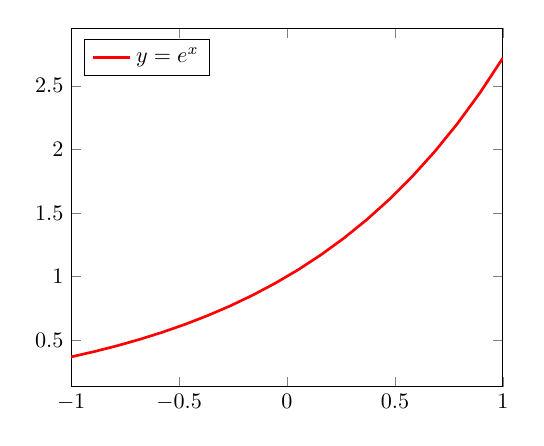
\begin{tikzpicture}[scale=0.8]
	\begin{axis}[legend pos=north west,xmin=-1, xmax=1,legend cell align={left},]
	\addplot[color=red, line width=1.2pt,samples=20,domain=-1:1] {e^x};\addlegendentry{$y=e^x$}
	\end{axis}
\end{tikzpicture}
\caption{XXX方法的性能}
\label{fig:template-example}
\end{figure}
